\documentclass[12pt,letterpaper]{amsart}
\usepackage{amsthm,amsfonts,amssymb,amsmath}
\usepackage{amsmath, bm}
\usepackage{tabularx}
\usepackage{graphicx} 
\usepackage{tikz}
\usetikzlibrary{patterns}
\usetikzlibrary{arrows.meta}
\usetikzlibrary{arrows}
\usepackage{amscd}
\usepackage{parskip}
\usepackage{enumitem}
\usepackage{comment}  \newcommand\T{\rule{0pt}{2.7ex}}       \newcommand\B{\rule[-1.2ex]{0pt}{0pt}} 
\hyphenation{Grothen-dieck}
\newcommand{\scr}{\scriptstyle}
\newcommand{\tclb}{\textcolor{blue}}
\newcommand{\tclr}{\textcolor{red}}
\newcommand{\svwtwo}{\textcolor{black}}
\newcommand{\svw}{\textcolor{black}}
\newcommand{\sheila}{\textcolor{black}}
\newcommand{\sheilaFeb}{\textcolor{black}}  \newcommand{\sheilaFebAgain}{\textcolor{magenta}}  \newcommand{\emn}{\textcolor{blue}}
\oddsidemargin=0in
\evensidemargin=0in
\textwidth=6.50in             

\headheight=10pt
\headsep=10pt
\topmargin=.5in
\textheight=8in

\newcommand{\bC}{\mathbb{C}}
\newcommand{\bN}{\mathbb{N}}
\newcommand{\bK}{\mathbb{K}}
\newcommand{\bP}{\mathbb{Z}_+} 
\newcommand{\bQ}{\mathbb{Q}}
\newcommand{\bR}{\mathbb{R}}
\newcommand{\bZ}{\mathbb{Z}}


\newcommand{\cA}{\mathcal{A}}
\newcommand{\cB}{\mathcal{B}}
\newcommand{\cC}{\mathcal{C}}
\newcommand{\cF}{\mathcal{F}}
\newcommand{\cG}{\mathcal{G}}
\newcommand{\cI}{\mathcal{I}}
\newcommand{\cJ}{\mathcal{J}}
\newcommand{\cK}{\mathcal{K}}
\newcommand{\cL}{\mathcal{L}}
\def\Q{{\mathbb Q}}

\newtheorem{theorem}{Theorem}[section]
\newtheorem{lemma}[theorem]{Lemma}
\newtheorem{corollary}[theorem]{Corollary}
\newtheorem{conjecture}[theorem]{Conjecture}
\newtheorem{proposition}[theorem]{Proposition}

\theoremstyle{definition}
\newtheorem{definition}[theorem]{Definition}
\newtheorem{example}[theorem]{Example}
\newtheorem{observation}[theorem]{Observation}
\newtheorem{algorithm}[theorem]{Algorithm}
\newtheorem{remark}[theorem]{Remark}

\newcommand{\poRI}{\preccurlyeq_{\mathcal{R}{\mathfrak{S}}^\ast _\alpha}}  \newcommand{\poA}{\preccurlyeq_{\mathcal{A}^\ast _\alpha}}  \newcommand{\poAbar}{\preccurlyeq_{\mathcal{\bar{A}}^\ast _\alpha} } \newcommand{\poRIcover}{\prec_{\mathcal{R}{\mathfrak{S}}^\ast _\alpha}}
\newcommand{\poI}{\preccurlyeq_{{\mathfrak{S}}^\ast _\alpha}} 
\newcommand{\poIcover}{\prec_{{\mathfrak{S}}^\ast _\alpha}} 




\newlength{\cellsize}
\cellsize=3ex


\newcommand\tableau[1]{
\vcenter{
\let\\=\cr
\baselineskip=-16000pt
\lineskiplimit=16000pt
\lineskip=0pt
\halign{&\tableaucell{##}\cr#1\crcr}}}


\newcommand{\tableaucell}[1]{{\def \arg{#1}\def \void{}\ifx \void \arg
\vbox to \cellsize{\vfil \hrule width \cellsize height 0pt}\else
\unitlength=\cellsize
\begin{picture}(1,1)
\put(0,0){\makebox(1,1)[c]{}}
\put(0,0){\line(1,0){1}}
\put(0,1){\line(1,0){1}}
\put(0,0){\line(0,1){1}}
\put(1,0){\line(0,1){1}}
\end{picture}\fi}}

\DeclareMathOperator{\sgn}{sgn}
\DeclareMathOperator{\SRHT}{SRHT}
\DeclareMathOperator{\SSYCT}{SSYCT}
\DeclareMathOperator{\DIRT}{DIRT}
\DeclareMathOperator{\cont}{cont}
\DeclareMathOperator{\comp}{comp}
\DeclareMathOperator{\rev}{rev}
\DeclareMathOperator{\sh}{sh}
\DeclareMathOperator{\set}{set}
\newcommand{\dI}{\mathfrak{S}^*}
\newcommand{\rdI}{\mathcal{R}\mathfrak{S}^*}
\newcommand{\CS}{\hat{\mathcal{S}}}
\newcommand{\RH}{\mathcal{RH}}
\newcommand{\Imtab}{\mathcal{I}}
\DeclareMathOperator{\QSym}{QSym}
\DeclareMathOperator{\Des}{Des}
\DeclareMathOperator{\DesI}{Des_{\dI}}
\DeclareMathOperator{\DesCS}{Des_{\CS}}
\DeclareMathOperator{\RS}{\mathcal{RS^{row}}}
\DeclareMathOperator{\DesRS}{Des_{\RS}}
\DeclareMathOperator{\rw}{rw}
\DeclareMathOperator{\stdz}{stdz}
\DeclareMathOperator{\inv}{inv}
\DeclareMathOperator{\Inv}{Inv}
\DeclareMathOperator{\F}{\mathcal{F}}  \DeclareMathOperator{\chr}{\mathrm{ch}}  \DeclareMathOperator{\bA}{\bar{\mathcal{A}}} \DeclareMathOperator{\bpi}{\bar{\pi}} 
\newcommand{\Sym}{\ensuremath{\operatorname{Sym}}}

\newcommand{\Qsym}{\ensuremath{\operatorname{QSym}}}
\newcommand{\qm}{M}				\newcommand{\qf}{F}				\newcommand{\qc}{C}				\newcommand{\qs}{{\mathcal{S}}}		\newcommand{\qsy}{\hat{\mathcal{S}}}	\newcommand{\DI}{{\mathfrak{S}}^\ast}	         \newcommand{\RI}{\mathcal{R}{\mathfrak{S}}^\ast} \newcommand{\rqsy}{\mathcal{R}\hat{\mathcal{S}}}	\newcommand{\SIT}{\ensuremath{\operatorname{SIT}}}
\newcommand{\SET}{\ensuremath{\operatorname{SET}}} \newcommand{\NSET}{\ensuremath{\operatorname{NSET}}}\newcommand{\SRCT}{\ensuremath{\operatorname{SRCT}}}

\newcommand{\Nsym}{\ensuremath{\operatorname{NSym}}}
\newcommand{\nce}{\mathbf{e}}         	\newcommand{\nch}{\mathbf{h}}         	\newcommand{\ncr}{\mathbf{r}}           	\newcommand{\ncs}{{\mathbf{s}}}          	\newcommand{\ncsy}{\hat{\mathbf{s}}}      \newcommand{\nci}{{\mathfrak{S}}}	         \newcommand{\ncri}{\mathcal{R}{\mathfrak{S}}} 
\newcommand{\NCSym}{\ensuremath{\operatorname{NCSym}}}
\newcommand{\slashp}{\mid}
\newcommand{\minel}{\hat{0}_n}
\newcommand{\maxel}{\hat{1}_n}
\newcommand{\mupi}{\mu_\Pi}
\newcommand{\mul}{\mu_L}
\newcommand{\bx}{\text{\bf x}}
\newcommand{\JT}{\mathrm{JT}}
\newcommand{\bdet}{\bm{\mathrm{det}}}
\newcommand{\id}{\mathrm{id}}
\newcommand{\st}{s^t}
\newcommand{\sort}{{\rm sort}}
\newcommand{\hig}{{\rm ht}}
\newcommand{\exch}{{\xi}}
\newcommand{\jota}{\mathcal{J}^t}
                   

\newcommand{\qalg}{\mathcal{Q}}   \newcommand{\qac}{q}                        
\newcommand{\palg}{\mathcal{P}}   \newcommand{\pmult}{\star}              
\newcommand{\ralg}{\mathcal{R}}

\newcommand{\calg}{\mathcal{C}\ell}
\newcommand{\ych}[1]{\xi^{#1}}         
\newcommand{\Sn}{\mathfrak{S}}

\newcommand{\qgrp}{\mathcal{F}}

\newcommand{\wsum}{\hat{\sigma}}
\newcommand{\wmax}{\omega}
\newcommand{\wmin}{\eta}
\newcommand{\hn}{H_n(0)}
\newcommand{\smodule}{\mathbf{S}}



\newcommand\ol[1]{\overline{#1}}
\newcommand\ul[1]{\underline{#1}}
\newcommand\ch[1]{\check{#1}}
\newcommand\strongof[1]{{#1}^+}
\newcommand\partitionof[1]{\widetilde{#1}}
\newcommand\reverse[1]{{#1}^*}
\newcommand\ccomplement[1]{{#1}^c}
\newcommand\ctranspose[1]{{#1}^t}

\newcommand{\des}{\mathrm{Des}} \newcommand{\desri}{\mathrm{Des}_{\mathcal{R}\mathfrak{S}^\ast}} \newcommand{\ninv}{\mathrm{inv}} \newcommand{\col}{\mathrm{col}} \newcommand{\rowrem}{\check{\mathfrak{h}}} \newcommand{\colrem}{\check{\mathfrak{v}}} \newcommand{\rem}{\check{\mathfrak{d}}} \newcommand{\rowremy}{\hat{\mathfrak{h}}} \newcommand{\colremy}{\hat{\mathfrak{v}}} \newcommand{\remy}{\hat{\mathfrak{d}}} \newcommand{\wcol}{w_{col}} \newcommand{\rT}{\check{T}} \newcommand{\rtau}{{T}} 
\newcommand{\refines}{\preccurlyeq}   \newcommand{\coarsens}{\succcurlyeq}   \newcommand{\fatzero}{\mathbf{0}}
\newcommand{\suchthat}{\;|\;}
\newcommand{\Subsetc}{\Subset _{\check{c}}}    \newcommand{\Subsetcy}{\Subset _{\hat{c}}}    \newcommand{\cskew}{{\!\!}}\newcommand{\cskewy}{{\!\!}_{\hat{c}}}\newcommand{\rhoc}{{\check{\rho}}} 
\newcommand{\rhocy}{{\hat{\rho}}} 
\newcommand{\Upsilonc}{{\check{\Upsilon}}} 
\newcommand{\Upsiloncy}{{\hat{\Upsilon}}} 
\newcommand{\cequiv}{\stackrel{c}{\sim}}    \newcommand{\yequiv}{\stackrel{y}{\sim}}    \newcommand{\Qequiv}{\stackrel{\tiny Q}{\sim}}   
\newcommand{\Pequiv}{\stackrel{\tiny P}{\sim}}   
\newcommand{\nearcat}{\odot}
\newcommand{\setnot}{\!\setminus\!}
\newcommand{\spam}{\operatorname{span}}
\newcommand{\cshape}{C\text{-}shape}
\newcommand{\pshape}{P\text{-}shape}
\newcommand{\rect}{\mathrm{rect}}

\DeclareFontFamily{U}{rcjhbltx}{}  \DeclareFontShape{U}{rcjhbltx}{m}{n}{<->rcjhbltx}{}
\DeclareSymbolFont{hebrewletters}{U}{rcjhbltx}{m}{n}
\DeclareMathSymbol{\shin}{\mathord}{hebrewletters}{152}


\author[Niese, Sundaram, van Willigenburg, Vega, Wang]{Elizabeth Niese, Sheila Sundaram, Stephanie van Willigenburg,\\ Julianne Vega, Shiyun Wang}

\address{Elizabeth Niese: Marshall University, Huntington, WV 25755, USA} 
\email{niese@marshall.edu}
\address{Sheila Sundaram: Pierrepont School, Westport, CT 06880, USA}
\email{shsund@comcast.net}
\address{Stephanie van Willigenburg: University of British Columbia, \svw{Vancouver,} BC V6T 1Z2, Canada}
\email{steph@math.ubc.ca}
\address{Julianne Vega: Kennesaw State University, \svw{Kennesaw, GA 30144,} USA}
\email{jvega30@kennesaw.edu}
\address{Shiyun Wang: University of Southern California, \svw{Los Angeles, CA 90089-2532,} USA}
\email{shiyunwa@usc.edu}

\title[Row-strict 0-Hecke algebra modules]{0-Hecke modules for row-strict dual immaculate functions}
\date{\today}

\begin{document}

\subjclass{\svw{05E05, 05E10, 06A07, 16T05, 20C08.}}
\keywords{\svw{Quasisymmetric functions, dual immaculate functions, 0-Hecke algebra, indecomposable module.}}

\begin{abstract}{We introduce a new basis of quasisymmetric functions, the row-strict dual immaculate functions.  We construct a cyclic, indecomposable 0-Hecke algebra module for these functions.   Our row-strict immaculate functions are related to the dual immaculate functions of Berg-Bergeron-Saliola-Serrano-Zabrocki (2014-15) by the involution  on the ring  of quasisymmetric functions.  We give an explicit description of the effect of  on the associated 0-Hecke modules, via the poset induced by the 0-Hecke action on standard immaculate tableaux.  This remarkable poset reveals other 0-Hecke submodules and quotient modules, often cyclic and indecomposable, notably for a row-strict analogue of the extended Schur functions studied in Assaf-Searles (2019). 

Like the dual immaculate function, the  row-strict dual immaculate function is the generating function of a suitable set of tableaux, corresponding to a specific  descent set. We give a complete combinatorial and representation-theoretic picture by constructing 0-Hecke modules for the remaining variations on descent sets,  and showing that \emph{all} the possible variations for generating functions of tableaux occur as characteristics of the 0-Hecke modules determined by these descent sets. }
\end{abstract}
\maketitle
\tableofcontents
\section{Introduction}\label{sec:Intro}
\svw{A recent flourishing area of research is that of Schur-like functions, whose properties are analogous to the ubiquitous Schur functions that arise in many areas, from enumerative combinatorics where they are generating functions for Young tableaux, to representation theory where they are the irreducible representations for the general linear groups, \sheila{as well as being intimately connected to representations of the symmetric group}.}

\svw{The area of Schur-like functions began with quasisymmetric Schur functions \cite{HLMvW2011},  followed by discoveries of row-strict quasisymmetric Schur functions \cite{MR2014}, Young quasisymmetric Schur functions \cite{LMvW2013, MN2015}, noncommutative Schur functions \cite{BLvW2011} and immaculate functions \cite{BBSSZ2014},  quasisymmetric Schur -functions \cite{JL2015},   quasisymmetric Macdonald polynomials \cite{CHMMW2022}, and Schur functions in noncommuting variables \cite{ALvW2021}.}

The results of this paper were  first announced in \cite{NSvWVW2022FPSAC}. 
In this paper and its companion \cite{NSvWVW2023}, we introduce a new family of quasisymmetric functions, the \emph{row-strict dual immaculate} functions.  Our focus in the present work is the study of the associated 0-Hecke algebra modules, which we define and analyse \svw{in order to develop the analogy with Schur functions in the representation theory context}. This programme was first carried out for the dual immaculate functions \cite{BBSSZ2015}, the quasisymmetric Schur functions \cite{TvW2015}, and subsequently for the row-strict Young quasisymmetric functions \cite{BS2021} and the extended Schur functions \cite{S2020}.

\svw{In further analogy with Schur functions, the row-strict dual immaculate functions  are  defined in  \cite{NSvWVW2023} as generating functions for certain types of tableaux of composition shape ; by identifying the correct descent set, it follows that the functions 
 expand positively in the basis of fundamental quasisymmetric functions, and are the image,} under the involutive algebra automorphism  of the Hopf algebra  of quasisymmetric functions, of the well-studied dual immaculate functions of \cite{BBSSZ2015}.

The descent set  determines a 0-Hecke algebra action on the set  of standard immaculate tableaux of composition shape , yielding a cyclic indecomposable module whose quasisymmetric characteristic is .  The action defines a partial order on the set  which turns out to be dual to the partial order in \cite{BBSSZ2015}, see Lemma~\ref{lem:sameposet}.  The resulting graded poset , which we call the immaculate Hecke poset,  has remarkable properties, leading to the discovery of several other 0-Hecke modules with interesting quasisymmetric characteristics.  Among these is an analogue of the extended Schur functions defined by Assaf and Searles \cite{AS2019}. An examination of the poset (see Figure~\ref{fig:Poset}) reveals various subposets that are closed under either our action or the dual immaculate action of \cite{BBSSZ2015}.  We  investigate the associated submodules.

One of the key contributions of this paper, then, is the 
careful scrutiny of the partial order resulting originally from the 0-Hecke algebra action defined in \cite{BBSSZ2015}, and the discovery that hidden within it are special standard immaculate tableaux, which generate interesting 0-Hecke algebra submodules and quotient modules, for both the dual immaculate action and our new row-strict dual immaculate action.
The duality in the poset reflects the action of the involution  on : we prove first that the poset is graded, and has unique top and bottom elements, see Definition~\ref{def:bot-elt} and Definition~\ref{def:top-elt}. The cyclic generator for the dual immaculate module was shown to be the top element in \cite{BBSSZ2015};  for the row-strict dual immaculate module, we show that  the cyclic generator is the  bottom element of the poset.  Similarly, the cyclic generators for the extended Schur Hecke-module of \cite{S2020} and our row-strict extended Schur Hecke-module (see Theorem~\ref{thm:Z-indecomp}) are the top and bottom elements of the interval , the column superstandard and row superstandard tableaux of   \svw{Definition~\ref{def:column-bot-elt} and Definition~\ref{def:top-elt}}, respectively.
Finally we show how another special standard tableau , see Definition~\ref{def:top-elt-SIT*}, also generates a cyclic submodule of the dual immaculate 0-Hecke algebra module.
The poset duality phenomenon can also be used to explain, for example, the passage between the modules in \cite{TvW2015} and \cite{BS2021}, see  Section~\ref{sec:dualImmsubmodules}. 

Our proofs are technical,  relying heavily on two  straightening algorithms which produce saturated chains in the poset    We prove  indecomposability by following the pioneering work in \cite{TvW2015} and  \cite{BBSSZ2015},  with considerable technical modifications.

The paper is organised as follows.  The basic definitions regarding quasisymmetric functions appear in Section~\ref{sec:Background}, which also includes the facts that we need about dual immaculate functions. Our new family of row-strict dual immaculate functions is introduced in Section~\ref{sec:RSImmFns}. In  Section~\ref{sec:Hecke-action-RSImm}, we briefly review the necessary facts about 0-Hecke algebras, and then define a new  0-Hecke algebra action on standard immaculate tableaux. Section~\ref{sec:partial-order} describes a partial order on these tableaux, which, by standard arguments, leads to a filtration showing that our 0-Hecke module has quasisymmetric characteristic equal to the row-strict dual immaculate function.

Section~\ref{sec:indecomp-module-and-poset} is devoted to showing that our new 0-Hecke module is cyclic (Theorem~\ref{thm:cyclic-rdI}) and indecomposable, culminating in Theorem~\ref{thm:Indecomp}.  The technicalities here hinge on two key straightening algorithms, described in Propositions~\ref{prop:bot-elt} and~\ref{prop:top-elt}, which we use to establish that the poset of Section~\ref{sec:partial-order} is bounded, with a unique minimal and maximal element.  The minimal element, defined in Definition~\ref{def:bot-elt}, is shown to be the cyclic generator of our module. The maximal element is the cyclic generator of the module of \cite{BBSSZ2015}.\footnote{It is not explicitly established in \cite{BBSSZ2015} that the poset of standard immaculate tableaux defined by the 0-Hecke action has a maximal element.} The straightening algorithms play an important role in the technical lemmas leading to the indecomposability proof.  The work of this section also reveals a remarkable connection, see  Lemma~\ref{lem:sameposet}, between our partial order and that of \cite{BBSSZ2015}, showing how the map  between the quasisymmetric characteristics of the dual immaculate and row-strict dual immaculate modules, is reflected in the duality of the posets.

The motivation for Section~\ref{sec:row-strict-ext} and Section~\ref{sec:dualImmsubmodules} comes from  a closer examination of the poset of standard immaculate tableaux defined by the 0-Hecke action, and the remarkable properties to which we have alluded above.  In Section~\ref{sec:row-strict-ext} we show how the poset reveals a 0-Hecke module whose characteristic is the row-strict analogue of the extended Schur function defined in \cite{AS2019}, for which a 0-Hecke module was constructed in \cite{S2020}.   In fact we show that there are not one but two related modules, a submodule  (Theorem~\ref{thm:Z-indecomp}) and a quotient module (Theorem~\ref{thm:another-bigone}) of the row-strict dual immaculate action, both cyclic and indecomposable.  To complete this analogy,  in Section~\ref{sec:dualImmsubmodules} we show once again how the poset of standard immaculate tableaux leads to the discovery of  more cyclic modules, a submodule and two quotient modules of the (original) dual immaculate action, as well as a quotient module of the extended row-strict dual immaculate module (Theorem~\ref{thm:dualImm-submodule-quotient}, Theorem~\ref{thm:SET-intersect-SIT*}).     Figure~\ref{fig:Poset} indicates the essential representation-theoretic properties of the immaculate Hecke  poset.

\sheila{We conclude in Section 9 by considering the two remaining choices for the descent set of a standard immaculate tableau, apart from the two which determine the dual immaculate and row-strict dual immaculate functions.  Although the corresponding quasisymmetric functions are no longer independent, interestingly, both of the new variants come with associated 0-Hecke actions.  Furthermore, these actions determine the same immaculate Hecke poset, and consequently our straightening algorithms apply, giving cyclic 0-Hecke modules as in Section~\ref{sec:indecomp-module-and-poset}, generated respectively by  and , as well as  submodules generated respectively by  and  as in  Section~\ref{sec:row-strict-ext} and  Section~\ref{sec:dualImmsubmodules}.} \sheilaFeb{Our final result, Theorem~\ref{thm:8flavours-tableaux}, shows that these modules complete the combinatorial picture of  tableaux  considered in this paper, by accounting for all the possible variations on increasing rows and columns.  This information is captured in Figure~\ref{fig:4-descent-sets}. }

\begin{figure}[htb] \centering
\scalebox{0.7}{	
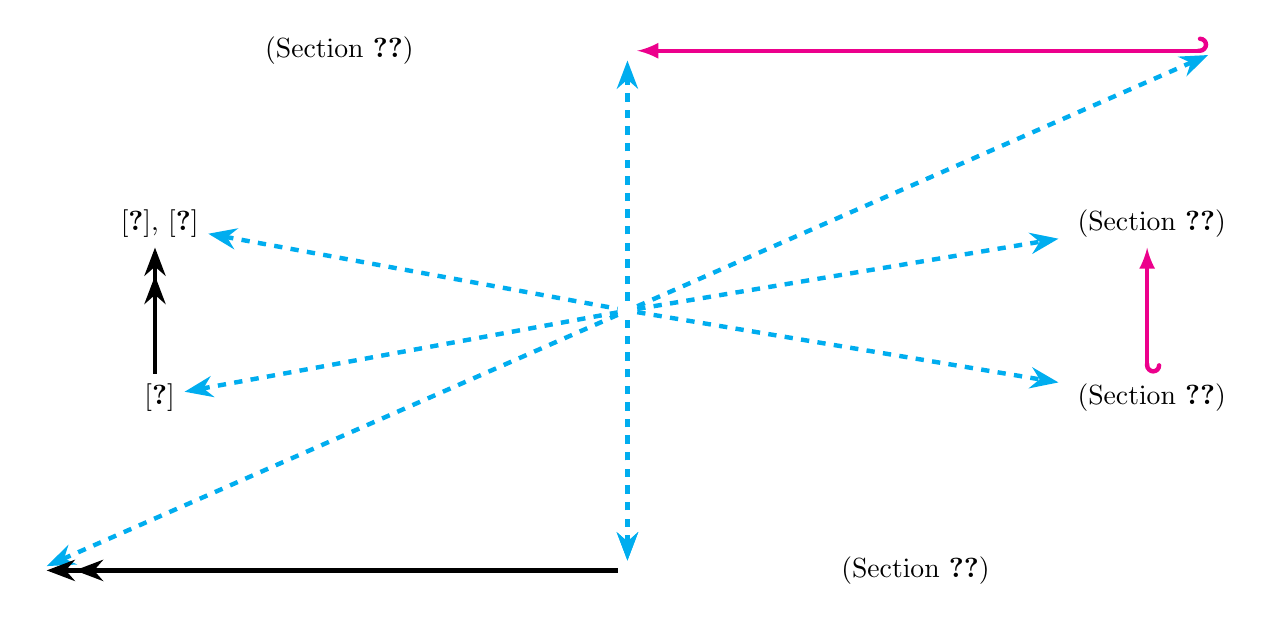
\begin{tikzpicture}\newcommand*{\xdist}{*3}
			\newcommand*{\ydist}{*2.2}
			\node (P0) at (0.00\xdist,0\ydist) {\tclb{}};
			\node (Q0) at (1.2\xdist, 0\ydist) {\ (Section~\ref{sec:new-descent-set})};
\node (P11) at (-2\xdist, 1\ydist) {\tclb{} \cite{BBSSZ2015}};
\node (P10) at (-2\xdist, 2\ydist) {\tclr{} \cite{S2020}, \cite{CFLSX2014}};
\node (P12) at (2.2\xdist, 2\ydist) {\tclb{} (Section~\ref{sec:RSImmFns})};
\node (P2) at (0\xdist, 3\ydist) { \tclb{}};
\node (Q2) at (-1.2\xdist, 3\ydist) {(Section~\ref{sec:new-descent-set})\ \  };
\node (P20) at (2.2\xdist, 1\ydist) {\tclr{} (Section~\ref{sec:row-strict-ext})};
\node (P3) at (0.00\xdist, 1.5\ydist) {};
\node (P01) at (-2.5\xdist , 0\ydist) {\tclr{ }};
\node (P22) at (2.5\xdist , 3\ydist) {\tclr{}};
\draw[ultra thick, magenta, left hook-latex] (P20) -- (P12);
\draw[ultra thick, -{Stealth}{Stealth}] (P11) -- (P10); 
\draw[ultra thick, dashed, cyan, {Stealth}-] (P11) -- (P3);
\draw[ultra thick, dashed, cyan, -{Stealth}] (P3) -- (P12);
\draw[ultra thick, dashed, cyan, {Stealth}-] (P10) -- (P3);
\draw[ultra thick, dashed, cyan, -{Stealth}] (P3) -- (P20);
\draw[ultra thick, dashed, cyan, {Stealth}-] (P0) -- (P3);
\draw[ultra thick, dashed, cyan, -{Stealth}] (P3) -- (P2);
\draw[ultra thick, dashed, cyan, {Stealth}-] (P0) -- (P3);
\draw[ultra thick, dashed, cyan, -{Stealth}]  (P3) -- (P01);
\draw[ultra thick, dashed, cyan, -{Stealth}]  (P3) -- (P22);
\draw[ultra thick, -{Stealth}{Stealth}] (P0) -- (P01);
\draw[ultra thick, magenta, left hook-latex] (P22) -- (P2);
\end{tikzpicture}
}
\caption{The eight flavours of tableaux, their characteristics and  -modules, related in pairs by the involution , from the four descent sets. The double arrow-head indicates a quotient module, and the hooked arrow indicates a submodule.}\label{fig:4-descent-sets}
\end{figure}

Table~\ref{table:standard-tableaux-acronyms} below provides a list of tableau  acronyms used in this paper.
\begin{table}[htbp]
\caption{Standard tableaux of composition shape  of , with distinct entries , where \textbf{all rows increase (strictly)  left to right}:}
\begin{center}
\scalebox{1}{
\begin{tabular}{|c|c|}
\hline
 & at least one column does NOT increase bottom to top\2pt]
 & first column filled bottom to top consecutively with \F_\alpha(x_1,x_2,\ldots) = \sum_{\substack{i_1\leq i_2\leq \cdots \leq i_n\\i_j<i_{j+1} \text{ if } j\in\set(\alpha)}} x_{i_1}x_{i_2}\cdots x_{i_n}.
\psi(F_\alpha) = F_{\alpha^c} \label{eqn:psiF}.
\DesI(S):=\{i: i+1 \text{ appears strictly above }i \text{ in } S \}.\Des_{\rdI}(S):=\{i:i+1\text{ is weakly below } i \text{ in } S\}.\rdI_\alpha = \sum_{S} F_{\comp(\Des_{\rdI}(S))} {s_i}^2 &=1; \\
               s_i s_{i+1}s_i &=s_{i+1}s_is_{i+1};\\
                  s_is_j &=s_js_i, \ |i-j|\ge 2.
 {\pi_i}^2 &=\pi_i; \\
               \pi_i\pi_{i+1}\pi_i &=\pi_{i+1}\pi_i\pi_{i+1};\\
                  \pi_i\pi_j &=\pi_j\pi_i, \ |i-j|\ge 2.
\label{eqn:HeckeIrreps} \pi_i(v_\alpha)=\begin{cases} 0, \ i\in \set(\alpha),\\
  v_\alpha, \text{ otherwise.}\end{cases}
 \mathrm{ch}([L_\alpha])= F_\alpha. \chr(\mathcal{W}_\alpha)= \dI_\alpha.\label{eqn:defn-dualImm-pi(T)}\pi_i^{\dI}(T)=\begin{cases} T, &\text{if  is in a row weakly below }i,\\
0,  & \text{if  are in column 1 of } T,\\
s_i(T), & \text{if  is strictly above  in },\\ &\text{and  are NOT in column 1},
\end{cases}\mathrm{Des}_{\dI}(T):=\{i: i+1 \text{ is strictly above } i \text{ in } T\}.\mathrm{ch}(\mathcal{W}_\alpha)=\dI_\alpha=\sum_T F_{\mathrm{comp}(\mathrm{Des}_{\dI}(T))},\label{eqn:defn-RSdualImm-pi(T)}\pi_i^{\rdI}(T)=\begin{cases} T, &\text{if } 
i\notin \mathrm{Des}_{\mathcal{R}\mathfrak{S^*}}(T), \\
0,& i\in \mathrm{Des}_{\mathcal{R}\mathfrak{S^*}}(T) \text{ and swapping } i \text{ and } i+1 \text{ in } T \\
\phantom{0,} & \text{does NOT result in a standard immaculate tableau},\\
s_i(T), & \text{otherwise},
\end{cases}S=\tableau{6\\4&5&8&10\\3&7\\1&2&9}.\pi^{\rdI}_i(T)=T \text{ for } i\in\{2,3,5,7,9\}, \ \ \pi^{\rdI}_1(T)=0=\pi^{\rdI}_4(T), \pi^{\rdI}_6(T)=s_6(T)=\tableau{{\bf 7}\\4&5& 8&10\\3& {\bf 6}\\1&2&9} , \quad  \pi^{\rdI}_8(T)=s_8(T)=\tableau{6\\4&5&  {\bf 9}&10\\3&7\\1&2& {\bf 8}}.\label{eqn:defn-pi(T)}\pi_i(T)=\pi_i^{\rdI}(T)=\begin{cases} T, & \text{if  is strictly above  },\\
0,  & \text{if  is right-adjacent to },\\
s_i(T), & \text{if  is strictly below  in }.
\end{cases}\label{eqn:keyclaim}\pi_i \pi_{i+1} \pi_i(T)=\pi_{i+1} \pi_i \pi_{i+1}(T).
\label{eqn:step1}\pi_i \pi_{i+1} ( s_i(T))= \pi_{i+1}(s_i(T)),
\label{eqn:step2} \text{In } s_i(T),  i+2 \text{ is now strictly above } i 
\text{ and weakly below }i+1. \label{eqn:step3} \text{In } s_i(T),  i+2 \text{ is now strictly above } i 
\text{ and strictly below }i+1. =\begin{cases} 0, & i+2 \text{ is right-adjacent to } i+1 \text{ in } T, \\
                          \pi_i(s_{i+1}(T)), 
                          &\text{otherwise.} \end{cases}=\begin{cases} 0, &i+2 \text{ is right-adjacent to } i+1 \text{ in } T, \\
                          \pi_{i+1}(\pi_i(s_{i+1}(T))), &\text{otherwise.} \end{cases}\pi_{i+1}\pi_i (s_{i+1}(T)).\label{eqn:step4} s_i s_{i+1} s_i(T) = s_{i+1} s_i s_{i+1}(T), \mathrm{Inv} (\sigma) = \{ (p,q)\suchthat 1\leq p < q \leq n \mbox{ and } \sigma(p) > \sigma (q)\}.\mathrm{Inv}(\sigma) = \{(1,2), (1,3), (1,4), (1,5),  (2,3), (2,4), (2,5), (3,5), (4,5)\}.\pi _i (T_1) = T_2\label{eq:inv}
\ninv (\sigma (T_2)) = \ninv (\sigma (T_1))+1.
T_1 \poRI T_2 \mbox{ if and only if there exists a permutation } s_{i_1} \cdots s_{i_\ell} \in S_n\pi _{i_1} \cdots \pi _{i_\ell} (T_1) = T_2.\ninv (\sigma (T_1)) \leq \ninv (\sigma (T_2))\ninv (\sigma (T_2)) \leq \ninv (\sigma (T_1)).\{\rtau _1 \poRI ^t  \cdots \poRI ^t \rtau _m  \}.\mathcal{V}_{\rtau_i} = \spam \{ \rtau _j \suchthat \rtau _i \poRI ^t \rtau _j \}\quad \text{ for } 1\leq i \leq m
\mathcal{V}_{\rtau_{m+1}}\subset \mathcal{V}_{\rtau_m} \subset \cdots \subset \mathcal{V}_{\rtau_{2}}\subset \mathcal{V}_{\rtau_1} 

\pi_{j}(\rtau_{i-1})&=& \left \lbrace \begin{array}{ll}0 & j\in \desri(\rtau_{i-1})\\\rtau_{i-1} & \text{otherwise.}\end{array}\right.

\mathrm{ch}(\mathcal{V}_\alpha)=\mathrm{ch}(\mathcal{V}_{\rtau_1})
&=& \displaystyle \sum_{i=2}^{m+1}F_{\comp(\desri(\rtau_{i-1}))}\nonumber\\ 
&=& \displaystyle \sum_{\rtau \in \SIT(\alpha)}F_{\comp(\desri(\rtau))}\nonumber\\ 
&=& \RI_{\alpha}.
\label{eqn:rdIcover} 
S\poRIcover  T
\iff \exists\, i \text{ such that }  T=\pi_i^{\rdI}(S),
\label{eqn:dIcover} 
S\poIcover  T
\iff \exists\, i \text{ such that }  S=\pi^{\dI}_i(T).
S\poIcover  T \iff S\poRIcover  T. S\poIcover  T&\iff \pi_i^{\dI}(T)=S, \text{ where }S\ne T, S\ne 0\\
& \iff i+1 \text{ is strictly above  in } T, \\ 
& \qquad\quad i, i+1 \text{ not both in column 1, by } \eqref{eqn:defn-dualImm-pi(T)}\\
&\iff i+1 \text{ is strictly BELOW  in } S\\
&\iff \pi_i^{\rdI} (S)=s_i(S)=T, \text{ by } \eqref{eqn:defn-pi(T)}\\
&\iff S\poRIcover  T.
S^0_{43423}=\tableau{\bf{5} &6 &7\\
                      \bf{4} &8\\
                      \bf{3}&9 & 10 & 11\\
                      \bf{2} & 12 & 13\\
                      \bf{1} & 14 & 15 & 16}\ , \qquad  
S^0_{43411}=\tableau{\bf{5} \\
                      \bf{4} \\
                      \bf{3}&6 & 7 & 8\\
                      \bf{2} & 9 & 10\\
                      \bf{1} & 11 & 12 & 13}\ .\label{eqn:fix-bot-elt}  
\pi_i^{\rdI}(S^0_\alpha)=S^0_\alpha\iff i\in [\ell-1].
\label{eqn:fix-bot-elt1}  
\pi_\ell^{\rdI}(S^0_\alpha)=0, \text { and }
\label{eqn:annihilate-bot-elt1}
 \pi_j^{\rdI}(S^0_\alpha)\notin \{S^0_\alpha, 0\}
 \iff j\in \{\ell+\alpha_\ell+\cdots+\alpha_{i}-(\ell-i+1), 2\le i\le \ell\}.
\label{eqn:annihilate-bot-elt2}
\pi_j^{\rdI}(S^0_\alpha)\notin \{S^0_\alpha, 0\}
\iff j=\ell \text{ or } j\in \{\ell+\alpha_\ell+\cdots+\alpha_{i}-(\ell-i+1),\, 2\le i\le k\}.
 S^0_\alpha \poRI T \text{ and } T=\pi_{j_1}\pi_{j_{2}}\cdots\pi_{j_r}(S^0_\alpha).\small{T=T_0\stackrel{\pi_4}{\longleftarrow} T_1=\tableau{\bf{4} &6 &7\\2 &5\\1&3}
 \stackrel{\pi_3}{\longleftarrow} T_2=\tableau{\bf{3} &6 &7\\2 &5\\1&4}}.T_2 \!  \stackrel{\pi_5}{\longleftarrow}\! T_3=\tableau{3 &\bf{5} &7\\2 &6\\1&4}\!\!\!
  \stackrel{\pi_4}{\longleftarrow} T_4=\tableau{3 &\bf{4} &7\\2 &6\\1&5}\!\!\!
  \stackrel{\pi_6}{\longleftarrow} T_5=\tableau{3 &4 &\bf{6}\\2 &7\\1&5}\!\!\!
 \stackrel{\pi_5}{\longleftarrow} T_6=\tableau{3 &4 &\bf{5}\\2 &7\\1&6}\!\!.
  T_6   \stackrel{\pi_6}{\longleftarrow} T_7=\tableau{3 &4 &5\\2 &\bf{6}\\1&7}=S^0_\alpha.
  T=\pi_4\pi_3\pi_5\pi_4\pi_6\pi_5\pi_6(S^0_\alpha).T\in \SIT(\alpha), T\ne S^0_\alpha\Rightarrow S^0_\alpha\poRI T,S^{row}_{43423}=\tableau{\bf{14} &15 &16\\
                      \bf{12} &13\\
                      \bf{8}&9 & 10 & 11\\
                      \bf{5} & 6 & 7\\
                      \bf{1} & 2 & 3 & 4}\ , \qquad 
                      S^{row}_{43411}=\tableau{\bf{13} \\
                      \bf{12} \\
                      \bf{8}&9 & 10 & 11\\
                      \bf{5} & 6 & 7\\
                      \bf{1} & 2 & 3 & 4}\ . T \poRI S^{row}_\alpha \text{ and } \pi_{j_r}\pi_{j_{r-1}}\cdots\pi_{j_1}(T)=S^{row}_\alpha.T_0\stackrel{\pi_4}{\longrightarrow} \tableau{3 &\bf{5} &7\\2 &6\\1 &4}\!\!\!\!=T_1
 \stackrel{\pi_5}{\longrightarrow}\tableau{3 &\bf{6} &7\\2 &5\\1 &4}\!\!\!\!=T_2
 \stackrel{\pi_3}{\longrightarrow} \tableau{\bf{4} &6 &7\\2 &5\\1 &3}\!\!\!\!=T_3
 \stackrel{\pi_4}{\longrightarrow} \tableau{\bf{5} &6 &7\\2 &4\\1 &3}\!\!\!\!=T_4.
 T_4   \stackrel{\pi_2}{\longrightarrow} \tableau{5 &6 &7\\\bf{3} &4\\1 &2}=S^{row}_\alpha.S^0_\alpha= T_1\preccurlyeq^t T_2 \preccurlyeq^t\dots \preccurlyeq^t T_m=S^{row}_\alpha,(0)\subset \mathrm{span}([S^0_\alpha, T_1])
\subset \dots \subset 
\mathrm{span}([S^0_\alpha, T_i])\subset \dots \subset \mathrm{span}([S^0_\alpha, S^{row}_\alpha]), (0)\subset\mathrm{span}([T_m,S^{row}_\alpha]) 
\subset\dots\subset \mathrm{span}([T_i,S^{row}_\alpha])\subset \dots \subset 
\mathrm{span}([S^0_\alpha, S^{row}_\alpha]).\binom{n}{2}+\binom{\ell}{3}-\sum_{i=1}^{\ell} \binom{\alpha_{i}+i-1}{2}f(S^0_\alpha)=\sum_{T\in \SIT(\alpha)} a_T T. f(S^0_\alpha)=\sum_{T\in \SIT^*(\alpha)} a_T T.j\in \Des_{\rdI}(P) \Rightarrow \pi_j(P)\ne P,  j\notin \Des_{\rdI}(S^0_\alpha) \Rightarrow \pi_j(S^0_\alpha)=S^0_\alpha.   f(S^0_\alpha)=f(\pi_j(S^0_\alpha))=\pi_j(f(S^0_\alpha))=\sum_T a_T \pi_j(T),a_P\ne 0 \Rightarrow 1, \ldots , \ell \text{ occupy the first column of } P,P\poRIcover P_1=\pi_\ell(P)\! \poRIcover P_2=\pi_{\ell-1}(P_1)\!\poRIcover
\cdots \!\poRIcover P_{\ell-i}=\pi_{i+1}(P_{\ell-i-1})P=\tableau{5 & 7 & 8\\ 4 & 10\\3 & 9\\2 &\bf{6} & 12\\1 & 11}\stackrel{\pi_5}{\longrightarrow} P_1=\tableau{6 & 7 & 8\\ 4 & 10\\3 & 9\\2 &\bf{5} & 12\\1 & 11}\stackrel{\pi_4}{\longrightarrow}
P_2=\tableau{6 & 7 & 8\\ 5 & 10\\3 & 9\\2 &\bf{4} & 12\\1 & 11}
\stackrel{\pi_3}{\longrightarrow}
P_3=\tableau{6 & 7 & 8\\ 5 & 10\\4 & 9\\2 &\bf{3} & 12\\1 & 11},Q=\tableau{5 & 7 & 8\\ 4 & 10\\3 & 9\\2 &11 & 12\\1 & \bf{6}}\stackrel{\pi_5}{\longrightarrow} Q_1=\tableau{6 & 7 & 8\\ 4 & 10\\3 & 9\\2 &11 & 12\\1 & \bf{5}}\stackrel{\pi_4}{\longrightarrow}
Q_2=\tableau{6 & 7 & 8\\ 5 & 10\\3 & 9\\2 &11 & 12\\1 & \bf{4}}
\stackrel{\pi_3}{\longrightarrow}
Q_3=\tableau{6 & 7 & 8\\ 5 & 10\\4 & 9\\2 &11 & 12\\1 & \bf{3}}\stackrel{\pi_2}{\longrightarrow}
Q_4=\tableau{6 & 7 & 8\\ 5 & 10\\4 & 9\\3 &11 & 12\\1 & \bf{2}};
\qquad \text{ hence for the sequence }\hat\pi=\pi_2\pi_3\pi_4\pi_5,\  \hat\pi(Q)=Q_4\ne 0.\text{Then } S^0_\alpha=\tableau{5 & 6 & 7\\4 &8\\3 &9\\2 &\bf{10} &11\\ 1 &12 &13};
\qquad \text{ we take } P=\tableau{5 & 6 & 7\\4 &8\\3 &9\\2 &12 &13\\ 1 &10 &11}.P \stackrel{\pi_9}{\longrightarrow} \tableau{5 & 6 & 7\\4 &8\\3 &10\\2 &12 &13\\ 1 &\bf{9} &11}
\stackrel{\pi_8}{\longrightarrow} \tableau{5 & 6 & 7\\4 &9\\3 &10\\2 &12 &13\\ 1 &\bf{8} &11}
\stackrel{\pi_7}{\longrightarrow} \tableau{5 & 6 & 8\\4 &9\\3 &10\\2 &12 &13\\ 1 &\bf{7} &11}
\stackrel{\pi_6}{\longrightarrow} \tableau{5 & 7 & 8\\4 &9\\3 &10\\2 &12 &13\\ 1 &\bf{6} &11},S^0_\alpha \stackrel{\pi_9}{\longrightarrow} \tableau{5 & 6 & 7\\4 &8\\3 &10\\2 &\bf{9} &11\\ 1 &12 &13}
\stackrel{\pi_8}{\longrightarrow}\tableau{5 & 6 & 7\\4 &9\\3 &10\\2 &\bf{8} &11\\ 1 &12 &13}
\stackrel{\pi_7}{\longrightarrow}\tableau{5 & 6 & 8\\4 &9\\3 &10\\2 &\bf{7} &11\\ 1 &12 &13}
\stackrel{\pi_6}{\longrightarrow}\tableau{5 & 7 & 8\\4 &9\\3 &10\\2 &\bf{6} &11\\ 1 &12 &13}\text{Let } S^0_\alpha=\tableau{\ell &\scriptstyle{\ell+1}\\ \ldots\\ \ldots\\ \ldots &\scriptstyle{p-1}\\ \ldots\\i & p\\
\ldots &\ldots\\
 j & \scriptstyle{y>p}\\
\ldots\\
\ldots &\ldots \\2\\1}\, ,\  
P=\tableau{\ell &\scriptstyle{\ell+1}\\  \ldots\\ \ldots\\ \ldots &\scriptstyle{p-1}\\ \ldots\\i &\scriptstyle{z>p}\\
\ldots &\ldots\\
 j & p\\
\ldots\\
\ldots &\ldots\\2\\1}\, .\ 
\text{ Then } \pi_{p-1}(P)=\tableau{\ell &\scriptstyle{\ell+1}\\  \ldots\\ \ldots\\ \ldots &\scriptstyle{p}\\ \ldots\\i 
& \scriptstyle{z>p}\\
\ldots &\ldots\\
 j & \scriptstyle{p-1}\\
\ldots\\
\ldots &\ldots\\2\\1}\, .\pi^{\rdI}_k(S)=T \iff S=\pi^{\dI}_k(T).T_1=\pi^{\dI}_{{i_r}}\pi^{\dI}_{{i_{r-1}}}\cdots \pi^{\dI}_{{i_1}} (U)  =T_2,f(S^0_\alpha) = \sum_{T\in \SIT^*(\alpha)} a_T T.\label{eq:thm:indecomp2}0=f(\hat\pi(S^0_\alpha))=\hat\pi(f(S^0_\alpha))
 =\sum_{T\in \SIT^*(\alpha)} a_T\ \hat\pi(T).r+\mathrm{rank}(\hat T)=\mathrm{rank}(T')=\mathrm{rank}(\hat\pi( T))\le r+\mathrm{rank}(T),f(S^0_\alpha)= a_{S^0_\alpha}\ S^0_\alpha;T_1=\tableau{\ldots &\ldots &x &\ldots &i\\ 
                 \ldots &\ldots &\ldots  \\
                 \ldots &\ldots &\scriptstyle{i+1} &\ldots &(y) &\ldots} \text{ and } 
T_2=\tableau{\ldots &\ldots &i &\ldots &(x)\\ 
                 \ldots &\ldots &\ldots  \\
                 \ldots &\ldots &y &\ldots &\scriptstyle{i+1} &\ldots}.
\pi^{\rdI}_i(T_2)=s_i(T_2)\in \SET(\alpha).\{\rtau _1\preccurlyeq^{t}_{\rdI} \cdots \preccurlyeq^{t}_{\rdI}\rtau _m=S^{row}_\alpha\} 
0\subset \mathcal{Z}_{\rtau_m} \subset \cdots \subset \mathcal{Z}_{\rtau_{2}}\subset \mathcal{Z}_{\rtau_1}=[\rtau_1,S^{row}_\alpha]=\mathcal{Z}_\alpha,
\mathcal{Z}_{\rtau_i} = \spam \{ \rtau _j \suchthat \rtau _i \poRI ^t \rtau _j \}=[T_i, S^{row}_\alpha]\quad \text{ for } 1\leq i \leq m.\chr(\mathcal{Z_\alpha})=\sum_{T\in\SET(\alpha)} F_{\comp(\Des_{\rdI}(T))}.\label{eq:ext-Schur} 
\mathcal{E}_\alpha= \sum_{T\in \SET(\alpha)} F_{\comp(\Des_{\dI}(T))}.
\{i : i \text{ is weakly to the right of  in T}\}.  i  \text{ weakly  right of } i+1 \iff 
i \text{ strictly below } i+1 \iff i\in \Des_{\dI}(T).\mathcal{R}\mathcal{E}_\alpha=\sum_{T\in\SET(\alpha)} F_{\comp(\Des_{\rdI}(T))} = \psi(\mathcal{E}_\alpha).T=\tableau{6 &7\\ \bf{3} & 4 & 5\\ 1 &2}\stackrel{\pi_2}{\leftarrow} T_1
=\tableau{\bf{6} &7\\ 2 & 4 & 5\\ 1 &3}
\stackrel{\pi_5}{\leftarrow} T_2=\tableau{\bf{5} &7\\ 2 & 4 & 6\\ 1 &3}
\stackrel{\pi_4}{\leftarrow} T_3=\tableau{\bf{4} &7\\ 2 & 5 & 6\\ 1 &3}\stackrel{\pi_3}{\leftarrow} T_4=\tableau{3 &\bf{7}\\ 2 & 5 & 6\\ 1 &4}
\stackrel{\pi_6}{\leftarrow} T_5=\tableau{3 &6\\ 2 & 5 & 7\\ 1 &4}=S^{col}_{232}, \text{and thus } 
  T=\pi_2\pi_5\pi_4\pi_3\pi_6(S^{col}_{232}).T=\tableau{5 &7\\ \bf{3} & 4 & 6\\ 1 &2}\stackrel{\pi_2}{\leftarrow} T_1
=\tableau{\bf{5} &7\\ 2 & 4 & 6\\ 1 &3}
\stackrel{\pi_4}{\leftarrow} T_2=\tableau{\bf{4} &7\\ 2 & 5 & 6\\ 1 &3}
\stackrel{\pi_3}{\leftarrow} T_3=\tableau{3 &\bf{7}\\ 2 & 5 & 6\\ 1 &4}\stackrel{\pi_6}{\leftarrow} T_4=\tableau{3 &6\\ 2 & 5 & 7\\ 1 &4}=S^{col}_{232}, \quad
 \text{and thus } 
  T=\pi_2\pi_4\pi_3\pi_6(S^{col}_{232}).\pi_j(S^{col}_\alpha)\ne S^{col}_\alpha \iff \text{  is at the top of a column in }S^{col}_\alpha.f(S^{col}_\alpha)=\sum_{T\in\SET(\alpha)} a_T T.f(S^{col}_\alpha)=f(\pi_j(S^{col}_\alpha))=\sum_{T\in \SET(\alpha)} a_T \pi_j(T),\{S^0_\alpha=\rtau _1\preccurlyeq^{\NSET^t}_{\rdI} \cdots \preccurlyeq^{\NSET^t}_{\rdI}\rtau _m  \}.\mathcal{\bar V}_{\rtau_i} = \spam \{ \rtau _j \suchthat \rtau _i \poRI^{\NSET^t} \rtau _j \}\quad \text{ for } 1\leq i \leq m
0\subset \mathcal{\bar V}_{\rtau_m} \subset \cdots \subset \mathcal{\bar V}_{\rtau_{2}}\subset \mathcal{\bar V}_{\rtau_1}.
\label{eq:new-ext-Schur}\overline{\mathcal{R}\mathcal{E}}_\alpha= \sum_{T\in \NSET(\alpha)\cap\SIT(\alpha)} F_{\mathrm{comp}(\Des_{\rdI}(T))}.\label{eqn:rdI-ext-diff} \rdI_\alpha-\overline{\mathcal{R}\mathcal{E}}_\alpha=\sum_{\rtau \in \SET(\alpha)}F_{\comp(\desri(\rtau))}.
\pi_{j}(\rtau_{i-1})&=& \left \lbrace \begin{array}{ll}0, & j\in \desri(\rtau_{i-1}),\\\rtau_{i-1}, & \text{otherwise,}\end{array}\right.

\mathrm{ch}(\mathcal{\bar V}_{\alpha})&=\displaystyle\sum_{i=2}^{m+1}\mathrm{ch}(\mathcal{\bar V}_{\rtau_{i-1}}/\mathcal{\bar V}_{\rtau_{i}})= \displaystyle \sum_{i=2}^{m+1}F_{\comp(\desri(\rtau_{i-1}))}\nonumber\\ 
&= \displaystyle \sum_{\rtau \in \NSET(\alpha)\cap\SIT(\alpha)}F_{\comp(\desri(\rtau))}= \overline{\mathcal{R}\mathcal{E}}_\alpha,
\rdI_\alpha= \sum_{\rtau \in \SIT(\alpha)}F_{\comp(\desri(\rtau))}.f(S^0_\alpha)=\sum_{T\in \NSET(\alpha)\cap\SIT(\alpha)} a_T T. f(S^0_\alpha)=\sum_{T\in \NSET(\alpha)\cap\SIT^*(\alpha)} a_T T.\mathcal{R}\mathcal{E}_\alpha=\sum_{T\in\SET(\alpha)} F_{\comp(\Des_{\rdI}(T))}  . \dI_\alpha-\mathcal{E}_\alpha=\sum_{T\in \NSET(\alpha)\cap\SIT(\alpha)}  F_{\comp(\Des_{\dI}(T))}.  \rdI_\alpha-\mathcal{R}\mathcal{E}_\alpha=\overline{\mathcal{R}{\mathcal{E}}}_{\alpha}= \sum_{T\in \NSET(\alpha)\cap\SIT(\alpha)} F_{\mathrm{comp}(\Des_{\rdI}(T))}.\hat\pi_{v}(u_0)=u_0, \qquad \text{but } \hat\pi_{v}(v)\ne v.\hat\pi_{v}(u_0)=0, \qquad  \text{but } \hat \pi_{v}(v)\ne 0.S^{row*}_{223}=S^{col}_{223}=\tableau{3 &6 &7\\2&5 \\1& 4}\!,\ 
S^{row*}_{332}=\tableau{3 &8 \\2 &6 &7 \\1 & 4 & 5}\ne S^{col}_{332},\  S^{row*}_{1323}
=\tableau{4 &8  &9 \\3 &7  \\2 & 5 & 6\\1}\ne S^{col}_{1323}.T=\hat\pi^{\dI}(S^{row*}_\alpha).\pi^{\dI}_i(T)=s_i(T)\notin \{ T,0\} \iff  i, i+1 \text{ are NOT in column 1 of  and  is strictly above  in }, T \poRI S^{row*}_\alpha \text{ and } \pi_{j_r}\pi_{j_{r-1}}\cdots\pi_{j_1}(T)=S^{row*}_\alpha.T_0\stackrel{\pi_5}{\longrightarrow} \tableau{3\\2 &4 &\bf{6} \\1  &5 & 7 & 8}\!\!=T_1
 \stackrel{\pi_6}{\longrightarrow}\tableau{3\\2 &4 &\bf{7} \\1  &5 & 6 & 8}\!\!=T_2
 \stackrel{\pi_7}{\longrightarrow} \tableau{3\\2 &\bf{4} &{8} \\1  &5 & 6 & 7}\!\!=T_3
 \stackrel{\pi_4}{\longrightarrow} \tableau{3\\2 &\bf{5} &{8} \\1  &4 & 6 & 7}\!\!\!=T_4,
 \text{and } T_4\stackrel{\pi_5}{\longrightarrow} \tableau{3\\2 &\bf{6} &{8} \\1  &4 & 5 & 7}\!\!\!=T_5
\stackrel{\pi_6}{\longrightarrow} \tableau{3\\2 &\bf{7} &{8} \\1  &4 & 5 & 6}\!\!\!=T_6=S^{row*}_\alpha.S^{col}_\alpha=\tableau{3\\2 & 5 & \bf{7}\\1 &4 &6 &8}\stackrel{\pi_7}{\longrightarrow} \tableau{3\\2 &\bf{5} &{8} \\1  &4 & 6 & 7}\!\!=U_1
\stackrel{\pi_5}{\longrightarrow} \tableau{3\\2 &\bf{6} &{8} \\1  &4 & 5 & 7}\!\!=U_2
\stackrel{\pi_6}{\longrightarrow} \tableau{3\\2 &{7} &{8} \\1  &4 & 5 & 6}\!\!=U_3=S^{row*}_\alpha.\chr(\mathcal{X}_\alpha)= \sum_{T\in \SIT^*(\alpha)} F_{\comp(\Des_{\dI}(T))}.\chr(\mathcal{W}_\alpha/\mathcal{X}_\alpha)
= \sum_{T\in \SIT(\alpha)\setminus \SIT^*(\alpha)} F_{\comp(\Des_{\dI}(T))}.f(S^{row}_\alpha)=\sum_{T\in\SIT(\alpha)\setminus\SIT^*(\alpha)} a_T T.\chr(\mathcal{X}_\alpha)= 
\sum_{k\ge \ell} e_{\ell-1}(x_1,\ldots,x_{k-1}) x_k h_{\bar{\alpha}}(x_k,x_{k+1},\ldots ) ,s_\lambda = \sum _{T\in \SET (\lambda)} F_{\comp (\DesI (T))}s_{\lambda/\mu} = \sum _{T\in \SET (\lambda/\mu)} F_{\comp (\DesI (T))}\{ i-\ell \suchthat i\in \DesI (T), i>\ell \} = \{ i \suchthat i\in \DesI (D_T) \}.s_{(1^{\ell -1})}(x_1,\ldots,x_{k-1})x_k=e_{\ell-1}(x_1,\ldots,x_{k-1}) x_ks_{D_T}(x_k,x_{k+1},\ldots )= h_{\bar{\alpha}}(x_k,x_{k+1},\ldots ).\pi^{\dI}_j(P)=0 \iff  j, j+1 \text{ are in column 1 of  }\iff j\in [\ell-1],\pi^{\dI}_j(P)=P \iff j+1 \text{ is weakly below  in .}\label{eqn:Steph} \chr(\mathcal{X}_\alpha/\mathcal{Y}_\alpha)=
\sum _{k\geq \ell} e_{\ell -1} (x_1, \ldots, x_{k-1}) x_k \mathcal{E}_{\overline{\alpha}} (x_k, \ldots),
\label{Sheila-Elizabeth2022Feb21}
 \chr(\mathcal{Z}_\alpha/R{\mathcal{Y}}_\alpha)=
\sum _{k\geq \ell} h_{\ell -1} (x_1, \ldots, x_k) x_k R\mathcal{E}_{\overline{\alpha}} (x_{k+1}, \ldots)
 f(S^{col}_\alpha)=\sum_{T\in [S^{col}_\alpha, S^{row*}_\alpha]} a_T T;\chr(\mathcal{X}_\alpha/\mathcal{Y}_\alpha)=\sum_{T\in \SET(\alpha)\cap\SIT^*(\alpha)} F_{\comp(\Des_{\dI}(T))}.\chr(\mathcal{Z}_\alpha/R\mathcal{Y}_\alpha)=\sum_{T\in \SET(\alpha)\cap\SIT^*(\alpha)} F_{\comp(\Des_{\rdI}(T))}.\label{eqn:defn-TvW(T)}\pi_i^{TvW}(T)=\begin{cases} T, & \text{if  is strictly right of },\\
0,  & \text{if  is strictly NW of, or in the same column as, },\\
s_i(T), & \text{if  is strictly SW of }.
\end{cases}\label{eqn:defn-RBS(T)}\pi_i^{revBS}(T)=\begin{cases} T, & \text{if  is weakly left of },\\
0,  & \text{if  is right-adjacent to },\\
s_i(T), & \text{if  is strictly right of  but not in the same row}.
\end{cases}\pi_i^{TvW}(T)=S \quad \iff \quad \pi_i^{revBS}(S)=T.
\pi_i^{TvW}(T)=S &\iff \text{ is strictly SW of  in }\\
&\iff \text{ is strictly NE of  in }\\
&\iff \pi_i^{revBS}(S)= s_i(S)=T.
 \chr({\mathcal{A}_\alpha})=
\sum_{T\in \SIT(\alpha)} F_{\comp(\Des_{\mathcal{A}^*}(T))}. \chr({\bA_\alpha})=
\sum_{T\in \SIT(\alpha)} F_{\comp(\Des_{\bA^*}(T))}.\sum_{T\in \SET(\alpha)}F_{\comp(\Des_{\mathcal{A}^*}(T))};\sum_{T\in \SET(\alpha)}F_{\comp(\Des_{\mathcal{\bA}^*}(T))}.\sum_{T\in \SIT^*(\alpha)}F_{\comp(\Des_{\bA^*}(T))} = \sum_{k\geq \ell} e_{\ell-1}(x_1,\cdots,x_{k-1})x_k e_\beta(x_k,\ldots)e_{\alpha_\ell - 1}(x_{k+1},\ldots).s_\lambda = \sum _{T\in \SET (\lambda)} F_{\comp (\DesI (T))}s_{\lambda/\mu} = \sum _{T\in \SET (\lambda/\mu)} F_{\comp (\DesI (T))}\{ i-\ell \suchthat i\in Des_{\bA^*}  (T), i>\ell \} = \{ i \suchthat i\in \DesI (\tilde{D}_T \cup C) \}.s_{(1^{\ell -1})}(x_1,\ldots,x_{k-1})x_k=e_{\ell-1}(x_1,\ldots,x_{k-1}) x_ks_{\tilde{D}_T}(x_k,\ldots) s_{(1^{\alpha _\ell -1})}(x_{k+1},\ldots)= e_\beta(x_k,\ldots)e_{\alpha_\ell - 1}(x_{k+1},\ldots).\label{eqn:Elizabeth2022Feb21-barA}
=\begin{cases}
\sum _{k\geq \ell} e_{\ell -1} (x_1, \ldots, x_{k-1}) x_k \chr(\bA_{\SET(\overline{\alpha})})(x_k,x_{k+1},\ldots), 
& \alpha \neq (1^m,n-m),\\
e_n, &\text{ otherwise},
\end{cases}
\label{eqn:Elizabeth2022Feb21-A}
=
\begin{cases}
\sum_{k\geq \ell} h_{\ell -1} (x_1, \ldots, x_{k})x_k\chr(\mathcal{A}_{\SET(\overline{\alpha})})(x_{k+1},\ldots), & \alpha \neq (1^m,n-m),\\
h_n, \text{ otherwise}.
\end{cases}
\dI_\alpha=F_{(1^{\ell-1}, n-\ell+1)}=F_\alpha,\  \rdI_\alpha=F_{(\ell, 1^{n-\ell})},  \ 
\chr(\mathcal{A}_\alpha)=F_{(n)},\ \chr({\bA}_\alpha)=F_{(1^n)}.\Des_{\mathcal{A}^*}(T)\subseteq \Des_{\rdI}(T), 
\quad \Des_{\bA^*}(T)\supseteq \Des_{\dI}(T),\label{eqn:standard-model-Hecke-action}
\pi_i(T)=\begin{cases}
T & \text{ if  is NOT a descent of },\\
s_i(T)  & \text{ if  is a descent of  and } s_i(T)\in ST(\alpha),\\
0 &\text{ otherwise}.
\end{cases}
\pi_i^{\mathcal{A}^*}(T)=\begin{cases} T, & \text{if } 
i\notin \Des_{\mathcal{A}^*}(T) \\
\phantom{T} &\iff i+1 \text{ strictly above or right-adjacent to  in } , \\
s_i(T), &  i\in \Des_{\mathcal{A}^*}(T) \iff i+1 \text{ strictly below  in }. \\
\end{cases}\label{eqn:keyclaim*}\pi_i \pi_{i+1} \pi_i(T)=\pi_{i+1} \pi_i \pi_{i+1}(T).
\label{eqn:step1*}\pi_i \pi_{i+1} ( s_i(T))= \pi_{i+1}(s_i(T)),
\label{eqn:step2*} \text{In } s_i(T),  i+2 \text{ is now weakly above } i 
\text{ and strictly below }i+1. \label{eqn:step11*}\pi_i(s_{i+1}(T))= \pi_{i+1}\pi_i(s_{i+1}(T)),
\label{eqn:step4*} s_i s_{i+1} s_i(T) = s_{i+1} s_i s_{i+1}(T), \pi_i^{{\mathcal A}^*}(T)\notin \{T, 0\} \iff \pi_i^{\rdI}(T)\notin \{T, 0\} .\pi_i^{{\mathcal A}^*}(T)=s_i(T)\iff \pi_i^{\rdI}(T)=s_i(T)\iff i+1 \text{ is strictly below  in },\{\rtau _1 \poA^t  \cdots \poA ^t \rtau _m  \}. 0\subset \mathrm{span}([T_m,S^{row}_\alpha]) 
\subset\dots\subset \mathrm{span}([T_i,S^{row}_\alpha])\subset \dots \subset 
\mathrm{span}([S^0_\alpha, S^{row}_\alpha]).\svw{\pi_i^{\mathcal{A}^*}}(T)=T\iff i\notin \svw{\Des_{\mathcal{A}^*}(T),}\bpi_i(T)=\pi_i^{\bA^*}(T)=\begin{cases} T, & 
i\notin \Des_{\bA^*}(T)\iff i+1 \text{ strictly below } i \text{ in } T, \\
0 & i+1 \text{  right-adjacent to  in } \\
&\text{ or  both in 1st column}, \\
s_i(T), &   i+1 \text{ strictly above  in }, \\
&\text{ and } i, i+1 \text{ not both in 1st column}. 
\end{cases}\label{eqn:keyclaim*barA}\bpi_i \bpi_{i+1} \bpi_i(T)=\bpi_{i+1} \bpi_i \bpi_{i+1}(T).
\label{eqn:barAstep2}\bpi_i \bpi_{i+1} s_i(T)=\bpi_{i+1} s_i(T).\label{eqn:step4bar*} s_i s_{i+1} s_i(T) = s_{i+1} s_i s_{i+1}(T), \pi_i^{{\bA}^*}(T)=s_i(T)\iff \pi_i^{\dI}(T)=s_i(T)\iff i+1 \text{ is strictly above  in , and  are not both in column 1},0\subset \mathrm{span}([S^0_\alpha, T_1])
\subset \dots \subset 
\mathrm{span}([S^0_\alpha, T_i])\subset \dots \subset \mathrm{span}([S^0_\alpha, S^{row}_\alpha]),\{\rtau _1 \poAbar^t  \cdots \poAbar ^t \rtau _m  \}\pi_i^{\bA^*}(T)=T\iff i\notin \Des_{\bA^*}(T),\dI_\alpha=\sum_{T\in  \mathcal{T}_\alpha({\text{1st col}<, \text{rows}\le})}  \mathrm{cm}(T), \text{ and } \rdI_\alpha=\sum_{T\in  \mathcal{T}_\alpha({\text{1st col}\le, \text{rows}<})}  \mathrm{cm}(T).\mathcal{E}_\alpha=\sum_{T\in  \mathcal{T}_\alpha({\text{cols}<, \text{rows}\le})}  \mathrm{cm}(T).\mathcal{R}\mathcal{E}_\alpha=\sum_{T\in  \mathcal{T}_\alpha({\text{cols}\le, \text{rows}<})}  \mathrm{cm}(T).\label{eqn:gf-A}
\sheilaFeb{\chr({\mathcal{A}_\alpha}) =\sum_{T\in \SIT(\alpha)} F_{\comp(\Des_{\mathcal{A}^*}(T))}=\sum_{T\in  \mathcal{T}_\alpha({\text{1st col}\le, \text{rows}\le})}  \mathrm{cm}(T)}.
\label{eqn:gf-barA}
\sheilaFeb{\chr(\bA_\alpha) =\sum_{T\in \SIT(\alpha)} F_{\comp(\Des_{\bA^*}(T))}=\sum_{T\in  \mathcal{T}_\alpha({\text{1st col}<, \text{rows}<})}  \mathrm{cm}(T)}.
\label{eqn:gf-A-SET}
\sheilaFeb{\chr(\mathcal{A}_{\SET(\alpha)})= \sum_{T\in \SET(\alpha)} F_{\comp(\Des_{\mathcal{A}^*}(T))}
=\sum_{T\in  \mathcal{T}_\alpha({\text{cols}\le, \text{rows}\le})}  \mathrm{cm}(T)}.
\label{eqn:gf-barA-SET}
\sheilaFeb{\chr(\bA_{\SET(\alpha)})=\sum_{T\in \SET(\alpha)} F_{\comp(\Des_{\bA^*}(T))} =\sum_{T\in  \mathcal{T}_\alpha({\text{cols}<, \text{rows}<})}  \mathrm{cm}(T)}.
2pt]\hline
 \bf{Rows left to right}
& weak &\tclb{strict  } \2pt]\hline\hline
Action of   in  
&  & \tclb{}\2pt]\hline\hline
 &  
& \tclb{}
 \2pt]\hline
  standard, &\text{ strictly above },& \tclb{}\2pt]\hline\hline
 \textcolor{blue}{Partial order on } &Poset &\tclb{ Poset }\2pt]\hline
Imm. module generated by& top element:   & \tclb{bottom  element: } \2pt]\hline\hline
Extended Schur fn basis &  \cite{AS2019} & \tclb{, }  \2pt]
Basis \tclb{} & (quotient of larger module) & \tclb{submodule of }\2pt]
Basis \tclb{}&  & \tclb{quotient of }\2pt]\hline\hline
Fundamental   &  Irreducible, one-dimensional\2pt]   \hline   Dual immaculate  &   Cyclic ()=, indecomp. \T\2pt]
\cite{BBSSZ2014} & \cite{BBSSZ2015}\2pt]

& acts on \2pt]\hline
Quasisymmetric Schur &   Indecomp. iff  is simple; \2pt]
 & composition tableaux  \2pt]\hline
Row-strict quasisym Schur & \2pt]
 & \cite[Chapter 4]{LMvW2013}, \cite{BS2021}\2pt]\hline
(Column-strict) Young quasisym function  & \2pt]
\cite{LMvW2013}  & \\
[2pt]\hline
Row-strict Young quasisym function  & Indecomp. iff  is simple;\2pt] 
 \cite{MN2015} & \cite{BS2021}\2pt]
 & acts on  \2pt]\hline\hline Row-strict Extended  Schur  & Cyclic , \textit{submodule} of , 
indecomp.; \T\2pt]
 \hline  Row-strict Extended Quotient Schur  & Cyclic  , \textit{quotient} of , indecomp.; \T \2pt]
\textcolor{red}{*NOT a basis*}    &  \\ 
\hline
 of Dual immaculate submodule& Cyclic , \textit{submodule} of ; 
\T\2pt]
\textcolor{red}{*NOT a basis*}    &  \\ [2pt]\hline
 of Dual immaculate quotient module& Cyclic , \textit{quotient} of ;
\T\2pt]
\textcolor{red}{*NOT a basis*}     &  \\ [2pt]\hline
The five functions in Section 9: & Cyclic modules   acting on ;\2pt]
Theorem~\ref{thm:8flavours-tableaux} and Figure~\ref{fig:4-descent-sets}& quotient module  of  acting on ;\2pt]\hline
\end{tabular}
}    
\end{center}
\label{table:QSymfunctions-modules}
\end{table}

\bibliographystyle{plain}
\bibliography{refs}
\end{document}
